\documentclass[conference]{IEEEtran}
\usepackage{graphicx}

% path gambar
\graphicspath{{./picture/}}

% JUDUL %%%%%%%%%%%%%%%%%%%%%%%%%%%%%%%%%%%%%%%%%%%%%%%%%%%%%
\title{Analisis Kekuatan Sinyal Menggunakan InSSIDer}

% PENULIS %%%%%%%%%%%%%%%%%%%%%%%%%%%%%%%%%%%%%%%%%%%%%%%%%%%
\author{Maranti Nainggolan\\
\textit{Fakultas Teknologi Informasi}\\
\textit{Institut Teknologi Batam}\\
Batam, Indonesia\\
Email: {1922001@student.iteba.ac.id}
}

\begin{document}

% untuk mengeluarkan judul dan author
\maketitle

% ABSTRAK %%%%%%%%%%%%%%%%%%%%%%%%%%%%%%%%%%%%%%%%%%%%%%%%%%
\begin{abstract}
Wi-Fi atau Wireless Fidelity merupakan teknologi jaringan tanpa kabel yang menggunakan frekuensi tinggi. Frekuensi yang digunakan oleh teknologi Wi-Fi berada pada spektrum 2,4 GHz dan beroperasi dengan menggunakan spesifikasi dasar IEEE 802.11. Wi-Fi telah menjadi terminologi umum yang digunakan oleh semua orang tetapi tidak banyak yang tahu tentang faktor kinerja dari jaringan Wi-Fi dan bagaimana semua perangkat dapat tetap terhubung dengan access points.
\end{abstract}

% kata kunci %%%%%%%%%%%%%%%%%%%%%%%%%%%%%%%%%%%%%%%%%%%%%%%%
\begin{IEEEkeywords}
Access point, InSSIDer, SSID, Wi-Fi.
\end{IEEEkeywords}

% pendahuluan %%%%%%%%%%%%%%%%%%%%%%%%%%%%%%%%%%%%%%%%%%%%%%
\section{PENDAHULUAN}
\vspace{0.3cm}

Teknologi WiFi atau yang lebih dikenal dengan Wireless LAN (WLAN) telah banyak diimplementasikan oleh masyarakat baik di dalam maupun di luar negeri. Selain untuk aplikasi privat,  WLAN juga banyak digunakan untuk aplikasi public (hotspot).

\vspace{0.4cm}

WLAN merupakan jaringan yang tidak tampak karena merupakan gelombang radio. Terutama bila frekuensinya terlalu berdekatan, atau hilang oleh daya gelombang radio yang lebih besar sehingga jaringan yang kita buat menjadi tidak efisien. Untuk itu diperlukan suatu software yang dapat digunakan untuk mencari informasi jaringan WLAN pada suatu area lebih spesifik dari scan biasa. Salah satu software yang dapat digunakan adalah inSSIDer.

\vspace{0.4cm}

InSSIDer merupakan software Wi-Fi scanner yang dapat mengidentifikasi SSID, RSSI (Received Signal Strength Indicator), security, dan pengaturan yang ada pada AP. Software ini dikembangkan oleh MetaGeek, LLC.

\vspace{0.3cm}

\section{PENJELASAN DARI TEORI}

\vspace{0.2cm}

Pada pembahasan ini, akan ditampilkan hasil analisa kekuatan
sinyal Wi-Fi pada suatu perumahan dengan menggunakan software InSSIDer.
dimana kita sebagai administrator jaringan yang akan melakukan instalasi jaringan WLAN (hotspot atau Wi-Fi) baru pada suatu wilayah, tentunya sebelum melakukan instalasi dan perancangan jaringan maka perlu dilakukan survey terhadap wilayah yang akan menjadi sasaran pemasangan jaringan tersebut.

\vspace{0.3cm}

\section{METODDOLOGI PENGERJAAN}

\vspace{0.2cm}
Lokasi Denah
\vspace{0.2cm}
\begin{figure}[h]
	\centering
	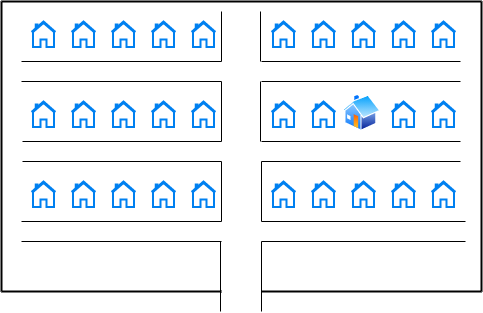
\includegraphics[width=0.2\textwidth]{Denah.png}
	\caption{Flowchart}
\end{figure}

\vspace{0.2cm}
Langkah Langkah Pengerjaan
\begin{enumerate}
    \item Menginstal aplikasi inSSIDer di Laptop.
    \item Menentukan tempat/sasaran yang akan dianalisa.
    \item Pengambilan data.
    \item Pengolahan dan analisa data yang didapat.
\end{enumerate}

\begin{figure}[h]
	\centering
	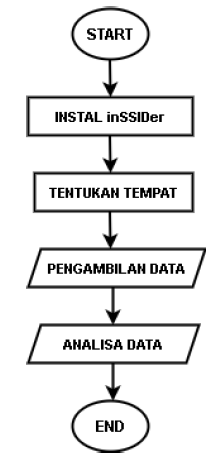
\includegraphics[width=0.2\textwidth]{Gambar1.png}
	\caption{Flowchart}
\end{figure}

\vspace{0.3cm}
Pada gambar 1 di bawah ini adalah tampilan inSSIDer saat bekerja.

\begin{figure}[h]
	\centering
	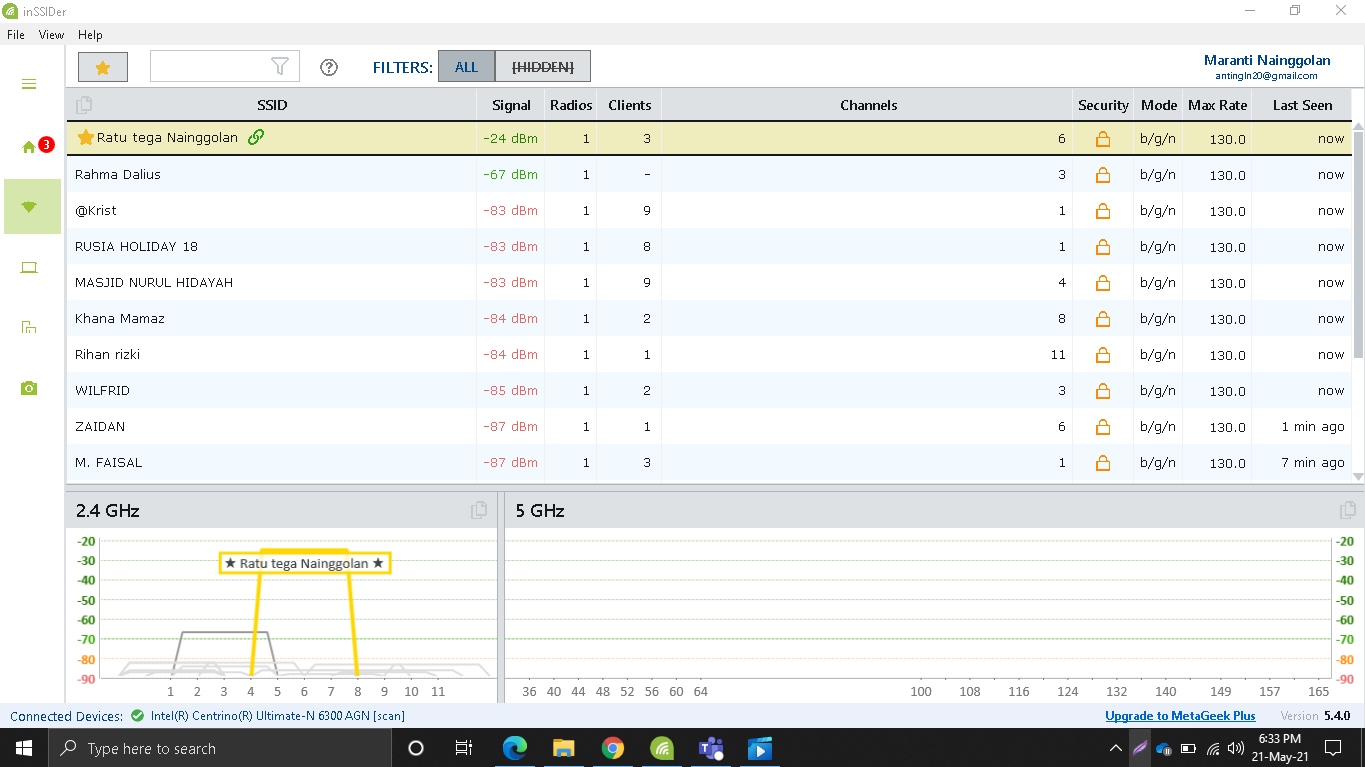
\includegraphics[width=0.4\textwidth]{2.png}
	\caption{Tampilan inSSIDer Saat Terhubung ke Internet}
\end{figure}

\begin{enumerate}
    \item Filters
    \vspace{0.2cm}
    
    Pada Bagian filter, terdapat Mode filter yang dapat
    digunakan yaitu antara lain: SSID, Signal, Radios, Client, Channels, Security, Mode, Max Rate, dan Last Seen.
    
    \begin{figure}[h]
        \centering
        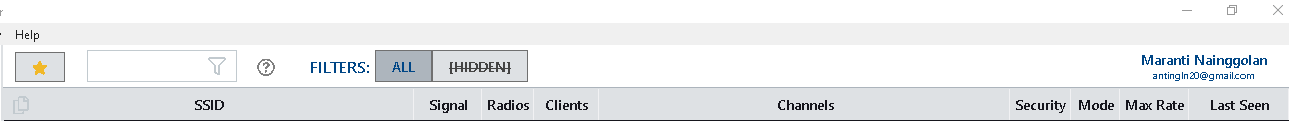
\includegraphics[width=0.4\textwidth]{3.png}
        \caption{Bagian - Bagian Filter}
    \end{figure}
    
    \vspace{0.2cm}
    
    \item SSID
    \vspace{0.2cm}
    
    Pada gambar dibawah, inilah beberapa list Network yang tertangkap atau yang ada disekitar perangkat saya.
    
    \begin{figure}[h]
        \centering
        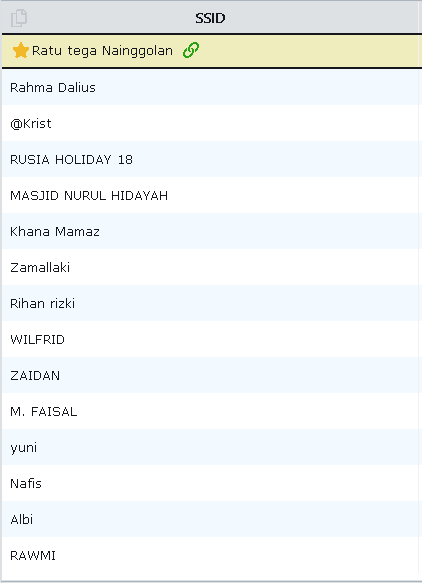
\includegraphics[width=0.3\textwidth]{4.png}
        \caption{List Network}
    \end{figure}
    \vspace{0.2cm}
    
    \item Signal, Radios, Client
    \vspace{0.2cm}
    
    Pada inSSIDer, kuat sinyal dapat dipantau secara detail dengan nilai pasti dalam satuan dBm. InSSIDer membagi klasifikasi kuat sinyal (dalam dBm).
    
    \begin{figure}[h]
        \centering
        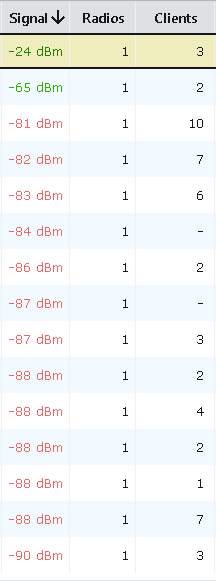
\includegraphics[width=0.1\textwidth]{5.png}
        \caption{Tampilan Signal, Radios, Client}
    \end{figure}
    \vspace{0.2cm}
    
    Kuat sinyal wifi akan sangat berpengaruh terhadap jarak, semakin jauh jarak akses point terhadap client maka semakin melemah pula kuat sinyal yang diterima oleh client.
    
    \begin{figure}[h]
        \centering
        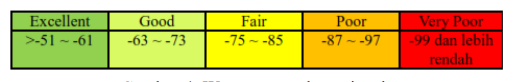
\includegraphics[width=0.3\textwidth]{6.png}
        \caption{Warna - Warna Kuat Sinyal}
    \end{figure}
    \vspace{0.2cm}
    
    Menurut gambar 6 tujuan yang harus dicapai supaya kualitas jaringan bisa optimal adalah dengan cara memposisikan akses point pada tempat yang tepat sehingga RSSI ( Received Signal Strength Indication ) yang di diterima sisi client dalam kondisi kuat (good dan excellent).
    
    \vspace{0.3cm}
    
    \item Chanels, Security, Mode, Max Rate, Last Seen
    
    \vspace{0.4cm}
    
    Dalam gambar dibawah terdapat ada channel, security (mekanisme keamanan), ada Mode, Max Rate (Kecepatan maksimal yang dapat digunakan) dan yang terakhir ada Last Seen.
    
    \begin{figure}[h]
        \centering
        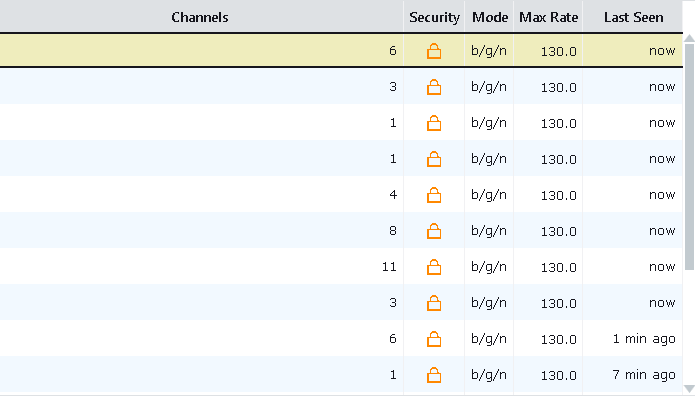
\includegraphics[width=0.5\textwidth]{7.png}
        \caption{Tampilan Chanels, Security, Mode, Max Rate, Last Seen}
    \end{figure}
    \vspace{0.2cm}
    \end{enumerate}
    
    \section{HASIL DAN PEMBAHASAN}
    \vspace{0.3cm}
    
    Pada tugas kali ini, dilakukan pengambilan data
    \begin{enumerate}
    \vspace{0.2cm}
    
        \item Pengambilan Data Didalah Rumah
        
    \begin{figure}[h]
        \centering
        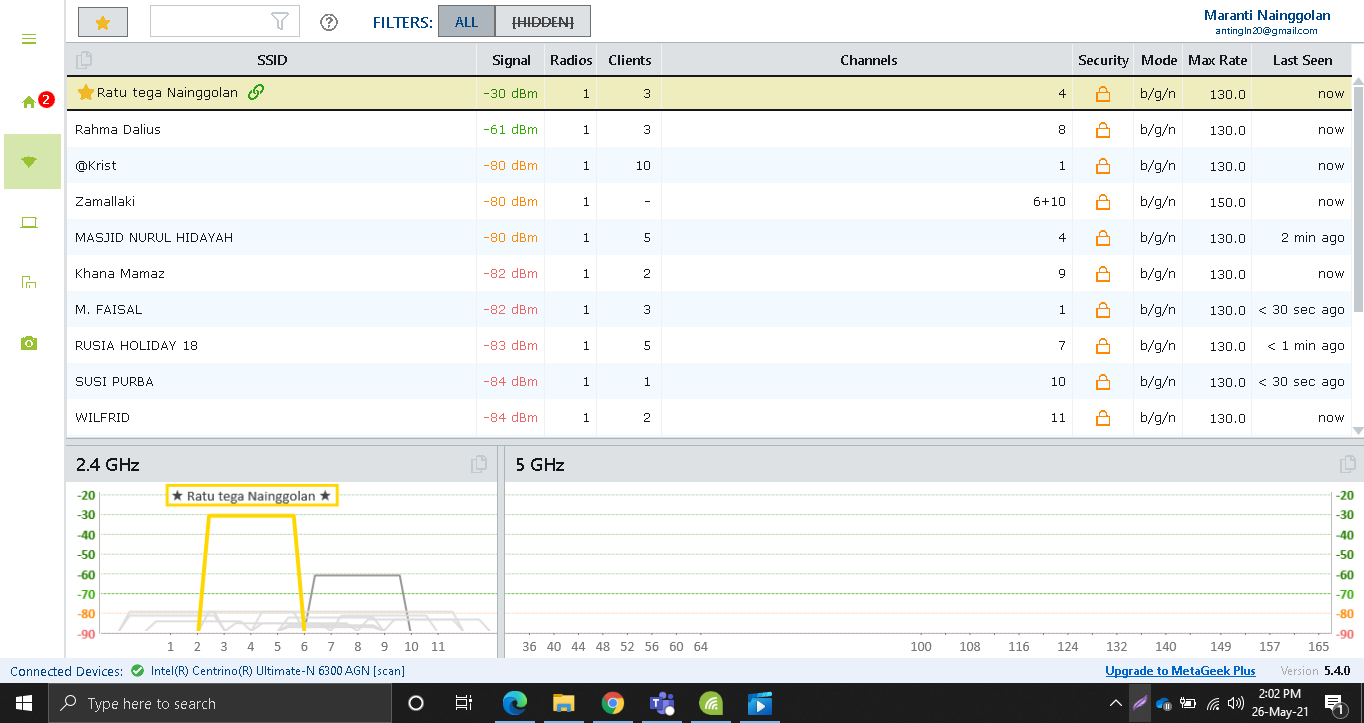
\includegraphics[width=0.4\textwidth]{8.png}
        \caption{Tampilan inSSIDer di Rumah}
    \end{figure}
    
    \begin{figure}[h]
        \centering
        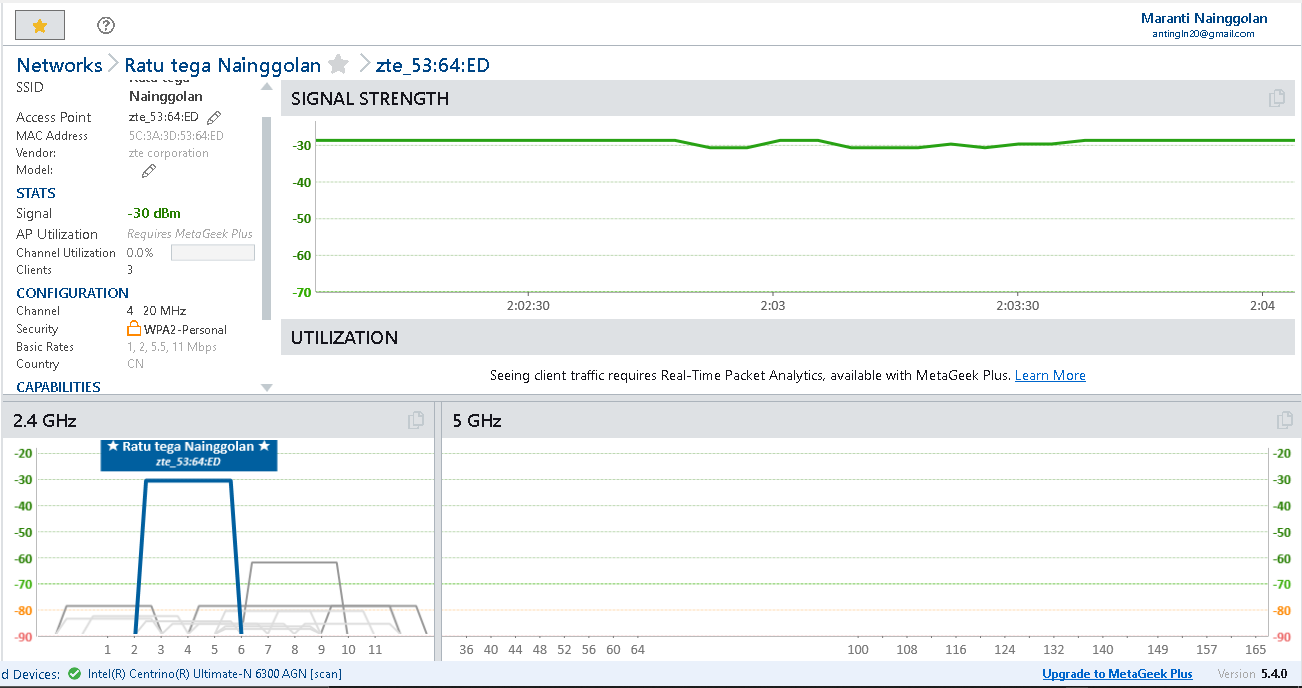
\includegraphics[width=0.4\textwidth]{9.png}
        \caption{Tampilan inSSIDer di Rumah}
    \end{figure}
    \vspace{0.3cm}
    
    Dari AP yang sinyalnya diterima dan terdeteksi pada inSSIDer terlihat bahwa AP dengan SSID Ratu Tega Nainggolan dirumah saya sendiri memiliki RSSI (Received Signal Strength Indicator) yaitu -30 dBm. Seting kanal yang digunakan adalah kanal 1 dan bekerja pada frekuensi 2,4 GHz. Menggunakan WPA-2 personal security, Client 3 dan memiliki channel 4.
    
    \vspace{0.3cm}
    
        \item Pengambilan Data Untuk jarak 15 meter Dari Rumah
        
    \begin{figure}[h]
        \centering
        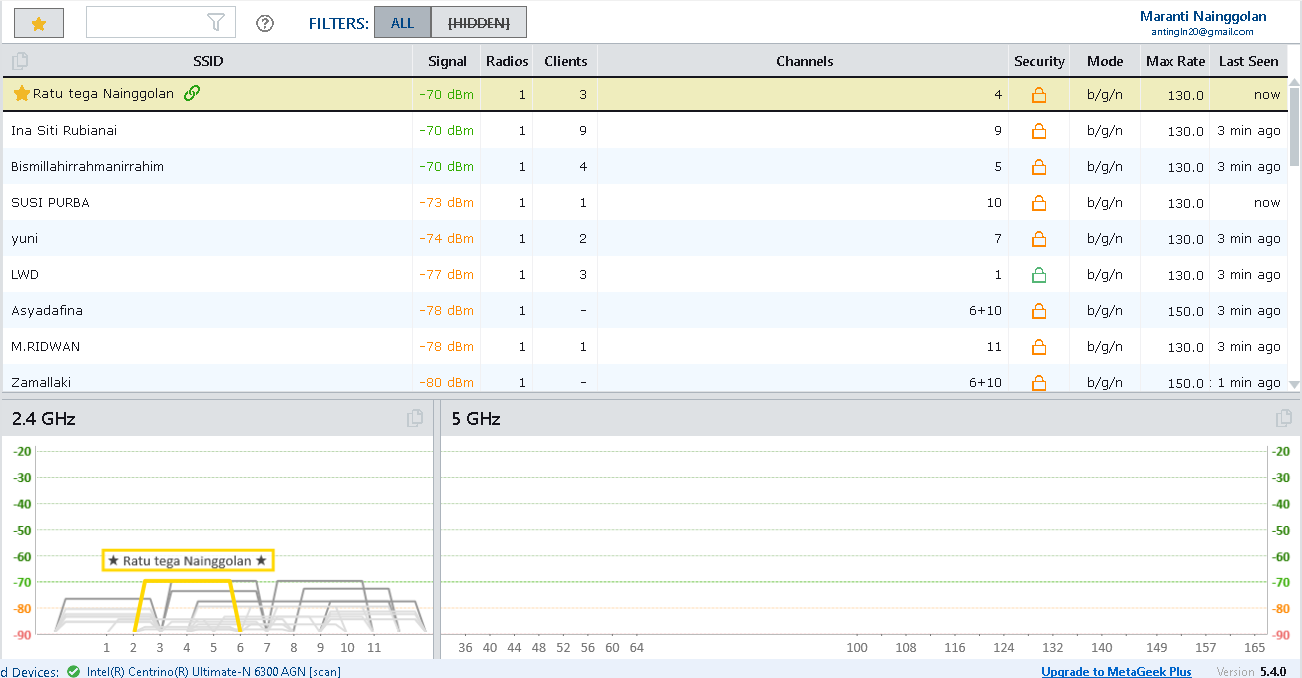
\includegraphics[width=0.4\textwidth]{10.png}
        \caption{Tampilan inSSIDer Dalam Jarak 15 Meter dari Rumah}
    \end{figure}
    
    \begin{figure}[h]
        \centering
        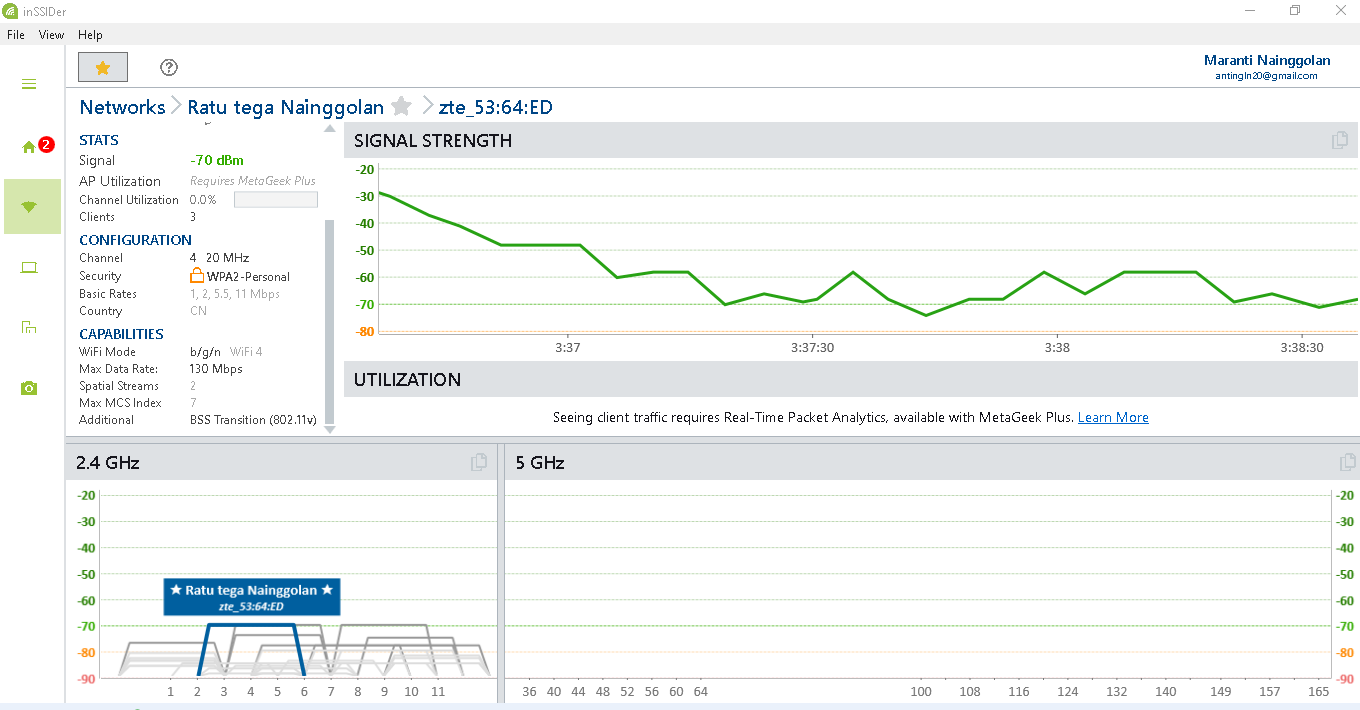
\includegraphics[width=0.4\textwidth]{11.png}
        \caption{Tampilan inSSIDer Dalam Jarak 15 Meter dari Rumah}
    \end{figure}
    \vspace{0.2cm}
    
    Pada gambar diatas terlihat bahwa sinyal wireless dengan SSID ‘Ratu Tega Nainggolan’ memiliki RSSI (Received Signal Strength Indicator) yakni -70 dBm. Berada pada kanal 1 dan bekerja pada frekuensi 2,4
    GHz. Menggunakan model WPA-2 personal security dan memiliki channel 4.
    \vspace{0.2cm}
    
        \item  Pengambilan Data dengan Adanya Penghalang / Pembatas (Dinding) 
    
    \begin{figure}[h]
        \centering
        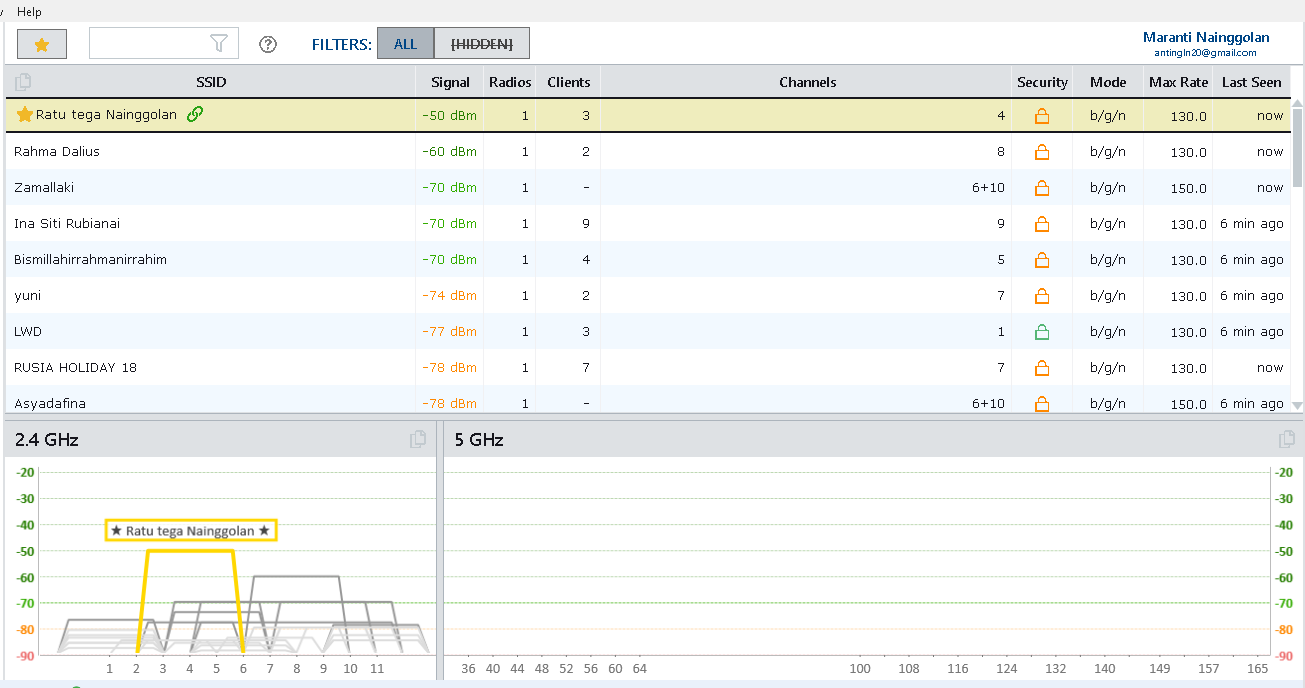
\includegraphics[width=0.4\textwidth]{12.png}
        \caption{Tampilan inSSIDer Dengan Adanya Pembatas}
    \end{figure}
    
    \begin{figure}[h]
        \centering
        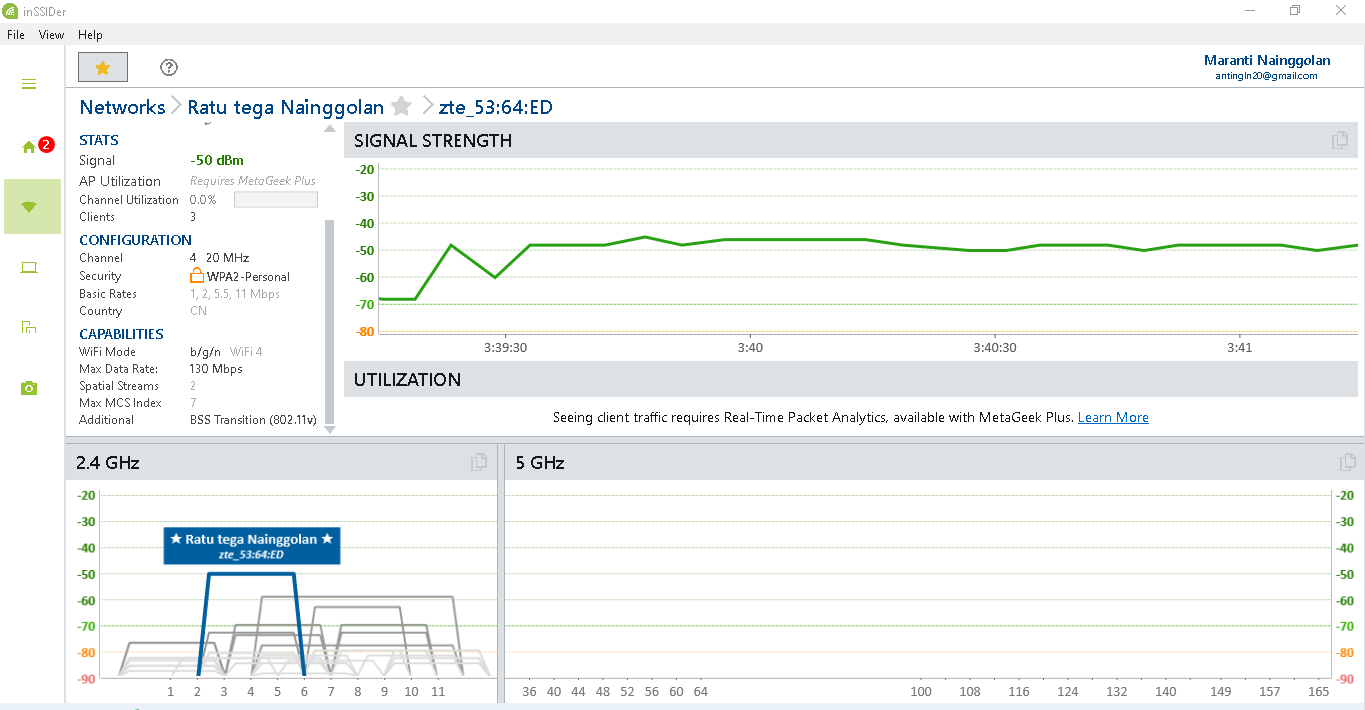
\includegraphics[width=0.4\textwidth]{13.png}
        \caption{Tampilan inSSIDer Dengan Adanya Pembatas}
    \end{figure}
    \vspace{0.2cm}
    
    Pada gambar 8 dan 9 terlihat bahwa sinyal wireless dengan SSID ‘Ratu Tega Nainggolan’ memiliki RSSI (Received Signal Strength Indicator) yakni -50 dBm. Berada pada kanal 1 dan bekerja pada frekuensi 2,4
    GHz. Menggunakan model WPA-2 personal security dan memiliki channel 4.
    \vspace{0.2cm}
    
    Dari semua gambar diatas dapat dilihat semua AP menggunakan atau bekerja di frekuensi 2.4 GHz. Frekuensi ini memang sering digunakan karena merupakan masuk dalam standard wireless 802.11b dan 802.11g. Sedangkan Pada data frekuensi 5 GHz tidak ada AP yang menggunakannya Terlihat pada panel 5GHz capture tidak ada SSID yang masuk kategori tersebut. Frekuensi 5GHz ini biasanya digunakan pada 802.11a yang notabennya memiliki max rate yang sama dengan 802.11g namun dengan pita yang lebih lebar.
    \end{enumerate}
    
    \vspace{0.2cm}
    \section{KESIMPULAN}
    \vspace{0.2cm}
    
    Pengambilan data untuk mengetahui kekuatan sinyal Wi-Fi dengan menggunakan inSSIDer telah dilakukan dengan baik. Dari semua gambar diatas dapat dilihat semua AP menggunakan atau bekerja di frekuensi 2.4 GHz. Frekuensi ini memang sering digunakan karena merupakan masuk dalam
    standard wireless 802.11b dan 802.11g. Sedangkan Pada data frekuensi 5 GHz tidak ada AP yang menggunakannya Terlihat pada panel 5GHz capture tidak ada SSID yang masuk kategori tersebut. Frekuensi 5GHz ini biasanya digunakan pada 802.11a yang notabennya memiliki max rate yang sama dengan 802.11g namun dengan pita yang lebih lebar.


% referensi %%%%%%%%%%%%%%%%%%%%%%%%%%%%%%%%%%%%%%%%%%%%%%%%
\begin{thebibliography}{00}
    \bibitem{b1} Pranjal., 2013, Experimental Study of a Wireless Local Area Network, International Journal of Information and Computation Technology, Vol.3 No. 10, pp.1047-1052
    \bibitem{b2} Julia Cynthia Rante, Max Alexander Rura Patras. Analisis Kekuatan Sinyal Vol. 14, No. 1, April 2018: 97-102 ISSN: 1907-0837
    \bibitem{b3} Eka, putra, daniel. 2013. Pengamatan Kuat Sinyal Access Point (AP) Menggunakan inSSIDer
    \bibitem{b4} Kapgate, Y., Vatti, R., Jadhav, S., 2017, WiFi Tools and Signal Strength Analysis, GRD Journals Global Research and Development Journal for Engineering , Vol.2 Issue 10.
\end{thebibliography}
\end{document}